\documentclass{article}
\usepackage[utf8]{inputenc}
\usepackage{hyperref}
\usepackage[letterpaper, portrait, margin=1in]{geometry}
\usepackage{enumitem}
\usepackage{amsmath}
\usepackage{booktabs}
\usepackage{graphicx}

\usepackage{titlesec}

\titleformat{\section}
{\normalfont\Large\bfseries}{\thesection}{1em}{}[{\titlerule[0.8pt]}]
  
\title{Homework 7}
\author{Economics 7103}
  
\begin{document}
  
\maketitle

\section{Python}
\noindent 1. If I understood correctly, this policy is directed towards manufacturers. Since we have data on car sales in 2017, I believe it most likely includes already assembled cars that were made before the policy came into force. That's why I think there will still be cars longer than 225 inches that do not have specific safety technology. Additionally, it takes time to readjust to such manufacturing requirements, and governments usually provide some transition time before the policy is fully implemented. So, I expect fuzzy RD.
\\

\noindent 2-5. The scatter plot of fuel efficiency in miles per gallon versus length is presented in Figure \ref{fig:scatterplot1}. There is bunching around the cutoff on both sides. It looks like a fuzzy RD, but I am not fully sure. However, definitely it is not a sharp RD. The fuel efficiency of the cars above the cutoff is smaller, as was expected by the new policy, but I suspect that long cars might have less fuel efficiency even without new policy-required technology. I think we should conduct robustness checks and McCrary test to confirm that this is proper fuzzy RD. The first-order polynomial fitted line is added to the scatter plot in Figure \ref{fig:scatterplot2}, the second-order in Figure \ref{fig:scatterplot3} and the fifth-order in Figure \ref{fig:scatterplot5}.  The first-stage treatment effect estimates are presented in Table \ref{tab:RD}. In the first column, the first-stage treatment effect is presented from the regression including a first-level polynomial. In the second column, results from the model with a second-level polynomial are displayed, and in the third column, the model with fifth-level polynomials is presented. The results from the first model, including the first-level polynomial, are statistically significant. Therefore, it is more reasonable to use only first-level fitting. In other cases, we face an overfitting issue.

\begin{figure}[h!]
    \centering
    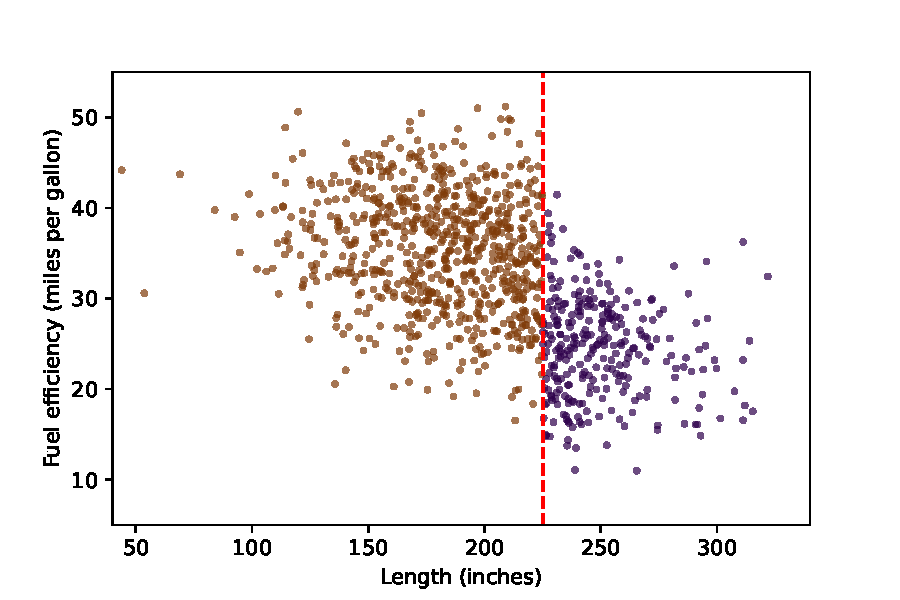
\includegraphics{homework 7/output/figure/scatterplot1.pdf}
    \caption{Scatter plot of Fuel efficiency in miles per gallon \& length}
    \label{fig:scatterplot1}
\end{figure}


\begin{figure}[h!]
    \centering
    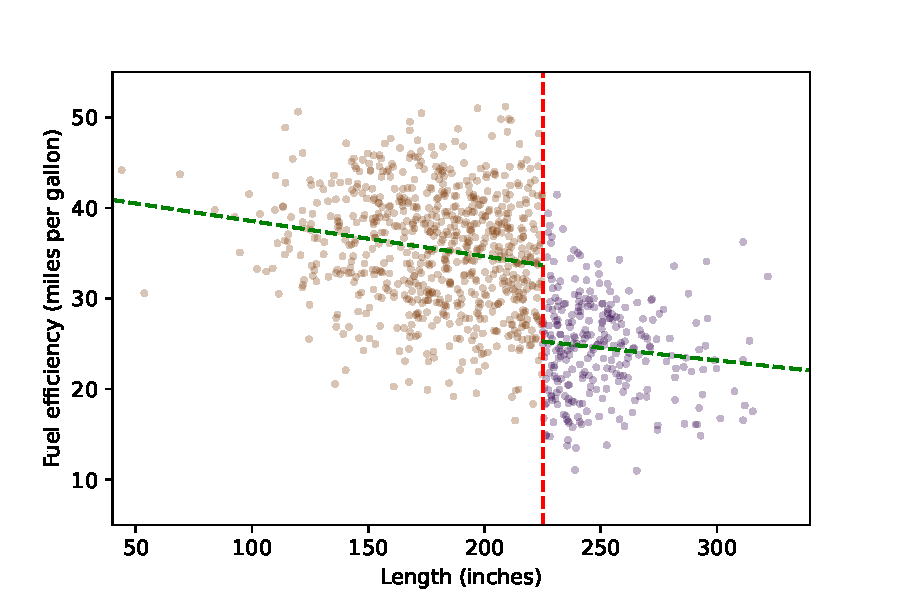
\includegraphics{homework 7/output/figure/scatterplot2.pdf}
    \caption{The first order polynomial.}
    \label{fig:scatterplot2}
\end{figure}


\begin{figure}[h!]
    \centering
    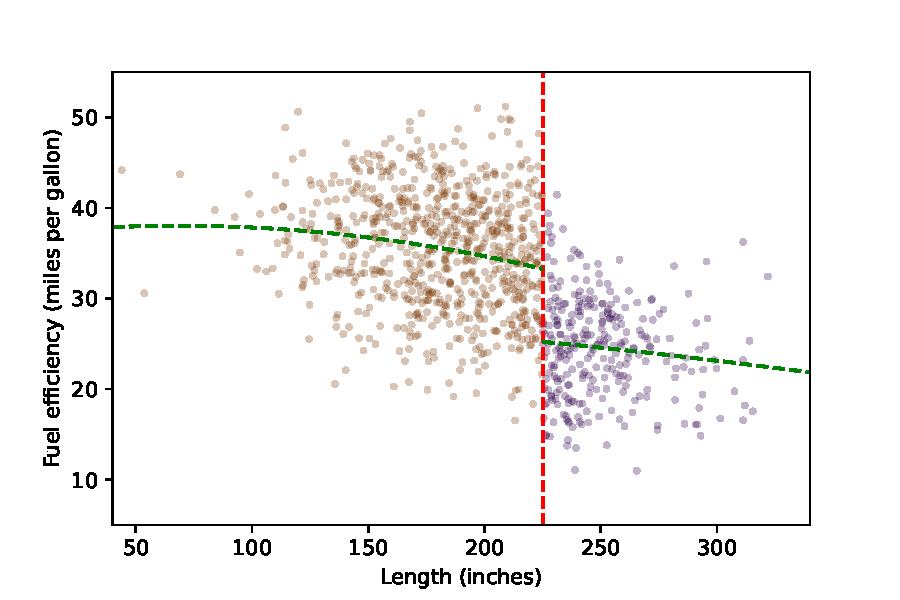
\includegraphics{homework 7/output/figure/scatterplot3.pdf}
    \caption{The second order polynomial.}
    \label{fig:scatterplot3}
\end{figure}


\begin{figure}[h!]
    \centering
    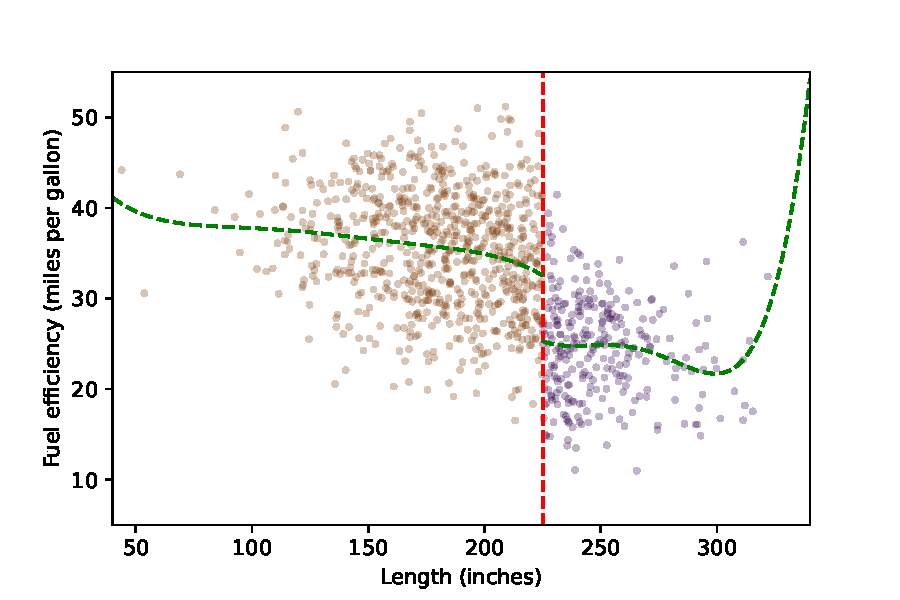
\includegraphics{homework 7/output/figure/scatterplot5.pdf}
    \caption{The fifth order polynomial.}
    \label{fig:scatterplot5}
\end{figure}



\begin{table}[h]
    \centering
    \begin{tabular}{@{\extracolsep{5pt}}lccc}
\\[-1.8ex]\hline
\hline \\[-1.8ex]
& \multicolumn{3}{c}{\textit{Dependent variable: mpg}} \
\cr \cline{2-4}
\\[-1.8ex] & (1) & (2) & (3) \\
\hline \\[-1.8ex]
  Treatment effect & -10.92$^{**}$ & -8.25$^{}$ & 0.38$^{}$ \\
& (4.50) & (46.30) & (0.34) \\
\hline \\[-1.8ex]
 Observations & 1000 & 1000 & 1000 \\
 $R^2$ & 0.40 & 0.40 & 0.40 \\
 Adjusted $R^2$ & 0.40 & 0.40 & 0.40 \\
 Residual Std. Error & 6.16 & 6.16 & 6.17 \\
 F Statistic & 259.65$^{***}$ & 162.43$^{***}$ & 248.22$^{***}$ \\
\hline
\hline \\[-1.8ex]
\textit{Note:} & \multicolumn{3}{r}{$^{*}$p$<$0.1; $^{**}$p$<$0.05; $^{***}$p$<$0.01} \\
\end{tabular}
    \caption{RD regression output}
    \label{tab:RD}
\end{table}
\clearpage

\noindent 6. It is more reasonable to use first-level polynomial in the first stage because as I mentioned in the previous section, treatment effect is statistically significant only in that case. 
\begin{table}[h]
    \centering
    \begin{tabular}{@{\extracolsep{5pt}}lccc}
\\[-1.8ex]\hline
\hline \\[-1.8ex]
& \multicolumn{3}{c}{\textit{Dependent variable: mpg}} \
\cr \cline{2-4}
\\[-1.8ex] & (1) & (2) & (3) \\
\hline \\[-1.8ex]
  Treatment effect & -10.92$^{**}$ & -8.25$^{}$ & 0.38$^{}$ \\
& (4.50) & (46.30) & (0.34) \\
\hline \\[-1.8ex]
 Observations & 1000 & 1000 & 1000 \\
 $R^2$ & 0.40 & 0.40 & 0.40 \\
 Adjusted $R^2$ & 0.40 & 0.40 & 0.40 \\
 Residual Std. Error & 6.16 & 6.16 & 6.17 \\
 F Statistic & 259.65$^{***}$ & 162.43$^{***}$ & 248.22$^{***}$ \\
\hline
\hline \\[-1.8ex]
\textit{Note:} & \multicolumn{3}{r}{$^{*}$p$<$0.1; $^{**}$p$<$0.05; $^{***}$p$<$0.01} \\
\end{tabular}
    \caption{2SLS regression output}
    \label{tab:2SLSRD}
\end{table}

\section{Stata}

\noindent 1.


\noindent 2. 

\end{document}